\chapter{Specifica dei requisiti}
Per la descrizione dei requisiti si è costruito un diagramma dei casi d'uso. I casi d'uso vengono poi descritti dettagliatamente.
\\Prima di iniziare a descrivere quali sono i casi d'uso, bisogna identificare gli attori che faranno parte del sistema.

\section{Attori Primari}
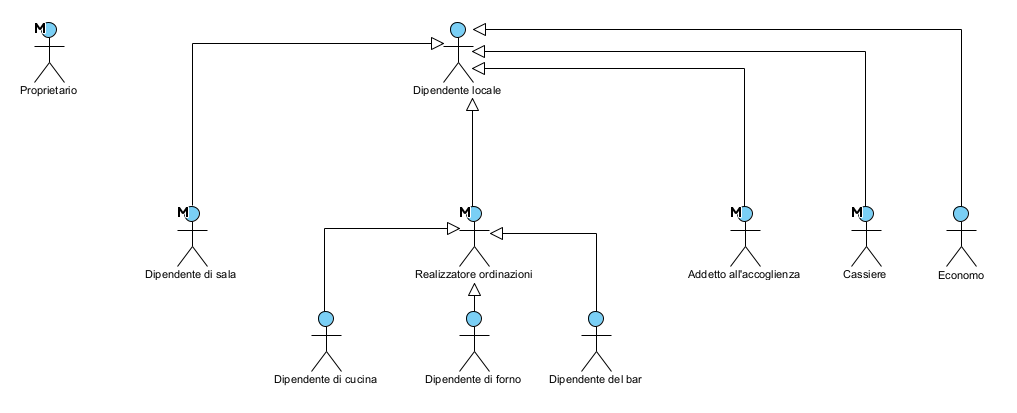
\includegraphics[width=\textwidth]{Immagini/AttoriPrimari.png}
\begin{itemize}
	\item Dipendente di sala: deve interagire con il cliente e prendere le ordinazioni in maniera tale che vengano smistate, tramite il sistema alle varie attività del locale
	\item Dipendenti di cucina/forno/bar: usano il sistema per ricevere i vari ordini e per notificare un completamento di essi
	\item Addetto all'accoglienza: usa il sistema per visualizzare i tavoli disponibili ed assegnarli ai clienti.
	\item Cassiere: richiede al sistema il conto totale di un cliente interessato per completare il pagamento
	\item Economo: si occupa della gestione delle merci ovvero l'aggiornamento delle quantità presenti in magazzino (in base alle vendite effettuate dalla sala e dalle richieste dei realizzatori di ordinazioni)
	\item Proprietario: può usare il sistema per aggiungere e rimuovere dipendenti, consultare dati come vendite, guadagni, quantità di merci.
\end{itemize}
Nella realtà tutti gli attori descritti non corrisponderanno tutti a persone fisiche differenti, infatti alcuni dipendenti possono assumere le funzionalità di più attori (ad esempio un dipendente di sala può anche ricoprire il ruolo di addetto all'accoglienza). A tal proposito quindi si è scelto di intendere gli attori sopra descritti come \textbf{ruoli} che un dipendente reale possa ricoprire.

\section{Attori Finali}
\begin{centering}
	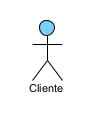
\includegraphics[width=0.15\textwidth]{Immagini/AttoriFinali.png}
\end{centering}

\begin{itemize}
	\item Cliente: pur non interagendo con il sistema, è direttamente interessato in alcuni suoi casi d'uso in quanto gli consentono di usufruire del servizio del locale
\end{itemize}

\section{Tabella Attori-Obiettivi}
Dopo aver identificato a pieno gli attori che utilizzeranno il sistema, bisogna associare ad ogni attore i suoi obiettivi.
\begin{table}[!h]
	\centering
	\begin{tabular}{|c || l|}
		\hline
		\rowcolor{Red}
		Attore & Obiettivi \\
		\hline
		\hline
		\multirow{9}{6em} {Proprietario} & Inserimento di un dipendente \\
		& Rimozione di un dipendente \\ & Modifica dei ruolo di un dipendente \\
		& Modifica dei tavoli e delle sale \\
		& Visualizzazione dei dipendenti \\
		& Inserimento di prodotti nel menu \\
		& Rimozioni di prodotti dal menu \\
		& Modifica di prodotti del menu \\
		& Visualizzazione del menu completo \\
		
		\hline
		\multirow{4}{6em} {Dipendente di sala} 
		& Creazione di un'ordinazione per un cliente  \\
		& Rimozione di un'ordinazione \\ 
		& Modifica di un'ordinazione \\
		& Visualizzazione di un'ordinazione per tavolo \\
		\hline
	
		\multirow{3}{6em} {Accoglienza} 
		& Assegnazione di un tavolo a dei clienti  \\
		& Modifica dello stato di un tavolo (libero, occupato, riservato, ecc.) \\ 
		& Visualizzazione di tutti i tavoli \\
		\hline	
		
		\multirow{2}{6em} {Cassiere} 
		& Visualizzazione degli ordini per tavolo  \\
		& Generazione vendita per un cliente\\ 
		\hline
		
		\multirow{2}{7em} {Realizzatore di ordinazione} 
		& Visualizzazione degli ordini per area (cucina, bar, forno)  \\
		& Notifica completamento ordinazione \\ 
		\hline
		
		\multirow{4}{6em} {Economo} 
		& Inserimento di una merce  \\
		& Modifica di una merce \\ 
		& Rimozione di una merce \\
		& Visualizzazione di una merce \\
		\hline
	\end{tabular}
\end{table}
Gran parte degli obiettivi riguardano operazioni CRUD (Create, Read, Update, Delete) che possono essere raggruppate in un solo obiettivo.
